\documentclass[jou]{apa6}

\usepackage[american]{babel}

\usepackage{csquotes}
\usepackage[style=apa,sortcites=true,sorting=nyt,backend=biber]{biblatex}
\DeclareLanguageMapping{american}{american-apa}
\addbibresource{bibliography.bib}


%%%%%%%%%%%%%%%%%%%%%%%%%%%%%%%%%%%%%%%%
%% Discrete Structures
%% The start of RBS stuff
%%%%%%%%%%%%%%%%%%%%%%%%%%%%%%%%%%%%%%%%

% Working internal and external links in PDF
\usepackage{hyperref}
% Extra math symbols in LaTeX
\usepackage{amsmath}
\usepackage{gensymb}
\usepackage{amssymb}
% Enumerations with (a), (b), etc.
\usepackage{enumerate}
\usepackage[framemethod=TikZ]{mdframed}
\usepackage{xcolor}

\let\OLDitemize\itemize
\renewcommand\itemize{\OLDitemize\addtolength{\itemsep}{-6pt}}

\usepackage{etoolbox}
\makeatletter
\preto{\@verbatim}{\topsep=3pt \partopsep=3pt }
\makeatother

% These sizes redefine APA for A4 paper size
\oddsidemargin 0.0in
\evensidemargin 0.0in
\textwidth 6.27in
\headheight 1.0in
\topmargin -24pt
\headheight 12pt
\headsep 12pt
\textheight 9.19in



\title{Sample Quiz 8}
\author{Discrete Structures, Spring 2020}
\affiliation{RBS}

\leftheader{Discrete Sample Quiz 8}

\abstract{%
}

%\keywords{}

\setlength\parindent{0pt}

\begin{document}

%\thispagestyle{empty}

\twocolumn
\section{Final Exam, 2020-04-23}

\vspace{4pt}
{\bf Question 1.}\\
By $U$ we denote the set of all positive integers 
between $1$ and $120$. This is the {\em universe} in which 
we define several subsets:
$$\left\{ \begin{array}{l}
A = \{ x \in U\;\mid\;2\mid{}x\},\\
B = \{ x \in U\;\mid\;3\mid{}x\},\\
C = \{ x \in U\;\mid\;5\mid{}x\},\\
X = \{ x \in U\;\mid\;2\mid{}x\;\vee\;3\mid{}x\},\\
Y = \{ x \in U\;\mid\;(3\mid{}x\;\wedge\;5\mid{}x)\;\vee\neg(2\mid{}x)\}.
\end{array} \right.$$

{\bf (A)} Express $X$ using the sets $A,B,C$ (using set union $V \cup W$, 
set intersection $V \cap W$, set complement $\overline{V}$ operations).\\
{\bf (B)} Express $Y$ using the sets $A,B,C$ in a similar way.\\
{\bf (C)} Find $|X|$ - the size of the set $X$.\\
{\bf (D)} Find $|Y|$ - the size of the set $Y$.




\vspace{10pt}
{\bf Question 2.}\\
Let $A$ and $B$ be sets with sizes $|A| = 8$ and $|B| = 5$
and $|A \cap B| = 3$. 

Calculate the largest and the smallest possible values 
for each of the following set sizes: 

{\bf (A)} $|A \cup B|$.\\
{\bf (B)} $|A \times (B \times B)|$.\\
{\bf (C)} $\left| \mathcal{P}(\mathcal{P}(A \cap B)) \right|$ - the 
powerset of a powerset of $A \cap B$.\\
{\bf (D)} $|A \oplus B|$ - the symmetric difference of the sets $A$ and $B$.


\vspace{10pt}
{\bf Question 3.}\\ 
Consider the following recurrent sequence: 

$$\left\{ \begin{array}{l}
a_0 = 3\\
a_1 = 4\\
a_{n+2} = 5a_{n+1} - 6a_n,\;\text{if}\;n \geq 0 \\
\end{array} \right.$$

Assume that $b_n$ is another sequence satisfying the 
recurrence rule
$$b_{n+2} = 5b_{n+1} - 6b_n,\;\text{if}\;n \geq 0$$
(The first two members $b_0,b_1$ are not known.)

{\bf (A)} Write the first $6$ members of this sequence ($a_0,\ldots,a_5$).\\
{\bf (B)} Write the characteristic equation for this sequence.\\
{\bf (C)} Write the general expression for an arbirary sequence $b_n$
satisfying the recurrent expression as a sum of two geometric progressions 
(you can leave unknown coefficients in your answer; just explain which ones they are).\\
{\bf (D)} Write the formula to compute $a_n$ (that would satisfy 
the initial conditions $a_0 = 3$ and $a_1 = 4$).


\vspace{10pt}
{\bf Question 4.}\\ 
Consider this code snippet in Python:

\begin{verbatim}
n = 1000
sum = 0
for i in range(1, n*n+1):
    for j in range(1,i+1):
        sum += i % j
\end{verbatim}

And a similar one in R:

\begin{verbatim}
n <- 1000
sum <- 0
for (i in 1:(n*n)) {
    for (j in 1:i) {
        sum <- sum + i %% j
    }
}
\end{verbatim}

{\bf (A)} Explain in human language what this algorithm does.\\
{\bf (B)} Denote by $f(n)$ the 
number of times the variable `sum` is incremented. 
Write the Big-O-Notation for $f(n)$. Find 
a function $g(n)$ such that 
$f(n)$ is in $O(g(n))$. (If there are multiple functions, 
pick the one with the slowest growth.)\\
{\bf (C)} Express the function $f(n)$ precisely - 
how many times `sum` is incremented in terms of variable $n$. 







\vspace{10pt}
{\bf Question 5.}

Let $A$ be the set of all positive divisors of the number $120$ 
(including $1$ and $120$ itself).  

{\bf (A)} What is the multiplication of all 
numbers in the set $A$?\\
{\bf (B)} Express this number as the product of prime powers.

 
 


\vspace{10pt}
{\bf Question 6.} 

Define the following binary relationship on the set of 
integer numbers $\mathbb{Z}$:   
We say that $aRb$ (numbers $a,b \in \mathbb{Z}$ are in the relation $R$) iff
$$\left\{ \begin{array}{l}
a - b \equiv 0\,(\text{mod}\;11)\\
a - b \equiv 0\,(\text{mod}\;12)\\
a - b \equiv 0\,(\text{mod}\;13)
\end{array} \right.$$

\begin{tabular}{|l|l|l|} \hline
{\bf Item} & {\bf Statement} & {\bf True or False?} \\ \hline
{\bf (A)} & $R$ is reflexive &  \\ \hline
{\bf (B)} & $R$ is symmetric &  \\ \hline
{\bf (C)} & $R$ is antisymmetric &  \\ \hline
{\bf (D)} & $R$ is transitive &  \\ \hline
{\bf (E)} & $aRb$ iff $a=b$ &  \\ \hline
\end{tabular}

For all items where you answered `FALSE`, specify a counterexample
(values for some numbers that would make the condition true, but the 
conclusion false). 
If the statement was true, write "none".


{\bf (A)} counterexample: $\ldots$\\
{\bf (B)} counterexample: $\ldots$\\
{\bf (C)} counterexample: $\ldots$\\
{\bf (D)} counterexample: $\ldots$\\
{\bf (E)} counterexample: $\ldots$


\vspace{10pt}
{\bf Question 7.}\\
Four people $A,B,C,D$ each has his own hat. 
After the meeting they leave their 
building in a hurry, everyone grabs some hat at random 
so that all $4!$ permutations of the hats have equal probabilities. 

Let the random variable $X$ denote the number of hats that
were picked up correctly. (For example, if
the hat assignment is this: $(A \rightarrow A, 
B \rightarrow B, C \rightarrow D, D \rightarrow C)$, then 
$X = 2$, because two people got their own hats.)

{\bf (A)}  Find $E(X)$ - the expected value of $X$.\\
{\bf (B)}  Find $V(X)$ - the variance of $X$. 



\vspace{10pt}
{\bf Question 8.}\\
There was a crooked man who had a crooked 1 euro coin. 
On lucky days it would flip the *heads* with probability $p=\frac{2}{3}$, 
and the *tails* with probability $p=\frac{1}{3}$, but on unlucky days
it was the opposite ($p(\mathtt{heads})=\frac{1}{3}$, but
$p(\mathtt{tails})=\frac{2}{3}$). 
There were equal probabilities of $\frac{1}{2}$ for lucky and unlucky days.


One morning he flipped the coin $5$ times and altogether got three {\em heads}
and two {\em tails}.

Let us introduce the following events:

\begin{itemize}
\item $E$ (evidence): Five coin tosses result in three {\em heads} and two {\em tails}.
\item $H$ (hypothesis): The current day is lucky.
\end{itemize}

{\bf (A)} Find $P(E|H)$ - the conditional probability of $E$ given that the 
day is lucky.\\
{\bf (B)} Find $P(E|H)\cdot P(H)$ - the probability that the day 
is lucky and $E$ happens.\\
{\bf (C)} Find $P(E|\overline{H})$ - the conditional probability of $E$
given that the day is not lucky.\\
{\bf (D)} Find $P(E|\overline{H})\cdot P(\overline{H})$ - the probability 
that the day is unlucky and $E$ happens.\\
{\bf (E)} Find $P(E)$ - as the sum of two probabilities ($E$ happened
on a lucky day and also $E$ happened on unlucky day).\\
{\bf (F)} Find the conditional probability $P(H|E)$ - 
the likelyhood that the croocked man has a lucky day, given 
that the event $E$ has happened.






\vspace{10pt}
{\bf Question 9.}

\begin{figure}[!htb]
\center{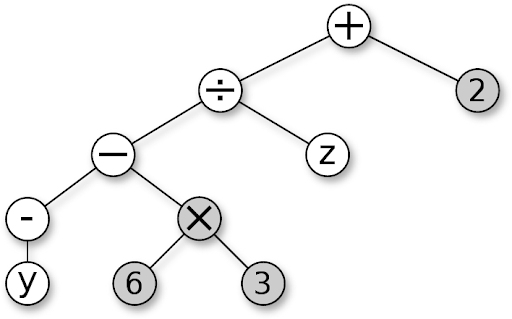
\includegraphics[width=2in]{final/final-syntax-tree.png}}
\caption{\label{fig:final-syntax-tree} A tree for an expression.}
\end{figure}

The syntax tree describes an algebraic expression (please note
the difference between the unary minus that
flips the value of the variable $y$ and 
the binary minus that subtracts the 
two subexpressions: $-y$ and $6 \times 3$). 

{\bf (A)} Write the preorder DFS traversal of
this tree.\\
{\bf (B)} Write the inorder DFS traversal of 
this tree.\\
{\bf (C)} Write the postorder DFS traversal of 
this tree.

{\em Note.} In all $3$ answers denote the unary 
minus with the tilde sign $\sim$, 
but the regular/binary minus with $-$. 






\vspace{10pt}
{\bf Question 10.}\\
\begin{figure}[!htb]
\center{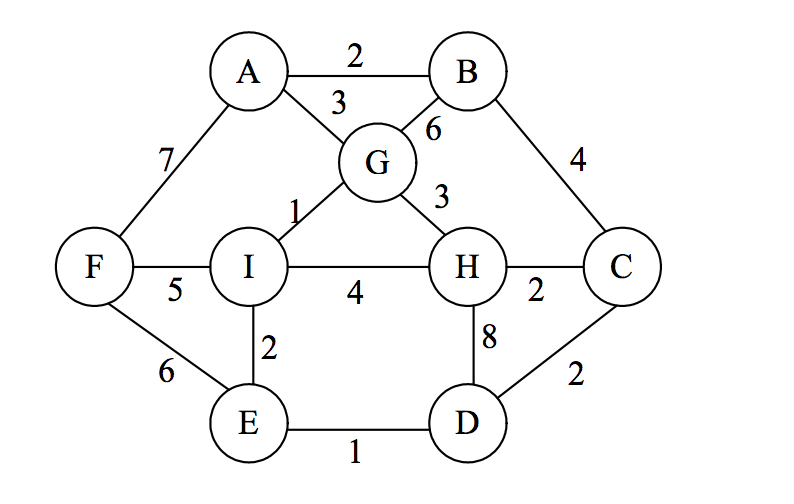
\includegraphics[width=2in]{final/prim-weighted-graph.png}}
\caption{\label{fig:prim-weighted-graph} A graph with 9 vertices.}
\end{figure}

Run the Prim's algorithm on the weighted graph in Figure~\ref{fig:prim-weighted-graph}, 
start growing the tree from the vertex $I$. 

\begin{tabular}{|l|l|} \hline
{\bf Step} & {\bf Newly Added Edge} \\ \hline
{\bf Step 1} & \\ \hline
{\bf Step 2} & \\ \hline
{\bf Step 3} & \\ \hline
{\bf Step 4} & \\ \hline
{\bf Step 5} & \\ \hline
{\bf Step 6} & \\ \hline
{\bf Step 7} & \\ \hline
{\bf Step 8} & \\ \hline
\end{tabular}


What is the total weight of the obtained Minimum Spanning Tree?





\mbox{}
\newpage
\subsection{Answers}

Every problem is worth $15$ points. The total for this final is 150 points.


\vspace{4pt}
{\bf Question 1.}\\

{\bf (A)} $X = A \cup B$ (Boolean OR means set union)\\
{\bf (B)} $Y = (B \cap C) \cup \overline{A}$ (Boolean and means set intersection; negation means set complement)\\
{\bf (C)} $|X| = |A| + |B| - |A \cap B| = 60+40-20 = 80$ (principle of inclusion-exclusion).\\
{\bf (D)} $|Y|$ is all odd numbers and also four even numbers divisible by $15$
($30, 60, 90, 120$). The total is $60 + 4 = 64$. 

{\scriptsize
{\em Grading.} 
\begin{itemize}
\item Each correct answer is $3$ points (total $12$). 
\item Explaining both {\bf (C}) and {\bf (D)} is another $3$ points (total $3$).
\item Using wrong set notation ($\wedge$ instead of $\cap$ etc.) divides the number of points in half.
\item $68$ instead of $64$ is $2$ points (instead of $3$). 
\end{itemize}
}


\vspace{10pt}
{\bf Question 2.}\\
In all the answers the largest and the smallest value are equal, because
we know exactly how the two sets intersect; how many elements belong to just
one of the sets $A$, $B$, and how many elements belong to the both sets. 

{\bf (A)} $|A \cup B| = |A| + |B| - |A \cap B| = 8+5-3 = 10$ (the principle of inclusion-exclusion).\\
{\bf (B)} $|A \times (B \times B)| = 8 \cdot 5 \cdot 5 = 200$\\
(Cartesian product has size that is the product of all participant sets: 
one can combine three elements from the sets $A$, $B$ and $B$ in this many ways).\\
{\bf (C)} $2^{2^3} = 2^8 = 256$ (the number of elements in the powerset 
of any set $X$ can be obtained by raising $2$ to the power $|X|$).\\
{\bf (D)} $|A \oplus B| = (8-3) + (5-3) = 7$ (we remove the common elements from both $A$ and $B$). 


{\scriptsize
{\em Grading.} 
\begin{itemize}
\item Each correct answer is $3$ points (total $12$).
\item Expressions or verbal explanations of the answers is $3$ points (total $3$).
\end{itemize}
}



\vspace{10pt}
{\bf Question 3.}\\
{\bf (A)} $a_0 = 3$,\\
$a_1 = 4$,\\
$a_2 = 5\cdot 4 - 6 \cdot 3 = 2$,\\
$a_3 = 5\cdot 2 - 6 \cdot 4 = -14$,\\  
$a_4 = 5\cdot(-14) - 6 \cdot 2 = -82$,\\
$a_5 = 5\cdot(-82) - 6 \cdot (-14) = -326$,\\
$a_6 = 5\cdot(-326) - 6 \cdot (-82) = -1138$.

{\bf (B)} The characteristic equation is obtained, if we try to find $a_n$ 
in the form of a geometric progression $r^n$:   
$r^{n+2} = 5r^{n+1} - 6r^n,$ or  
$r^2 -5r + 6 = 0$.   
It has two roots: $r_1 = 2$, $r_2 = 3$. 

{\bf (C)} The general form of the expression for any iterative
sequence $b_n$ satisfying the relationship $b_{n+2} = 5b_{n+1} - 6b_n$ is as follows:
$$b_n = A \cdot 2^n + B \cdot 3^n,$$
where $A,B$ are two constants that depend on the two initial values of the sequence $b_n$. 

{\bf (D)} We need to solve a system of two equations, to ensure that the formula
$a_n = A \cdot 2^n + B \cdot 3^n$ has correct values for $n=0$ and $n=1$. 
We get the following system: 
$$\left\{ \begin{array}{l} 
A + B = 3,\\
2A + 3B = 4.\\
\end{array} \right.$$
Substitute $B = 3-A$ into the second equation. We get that 
$2A + 9 - 3A = 4$ and $A = 5$. We also get that $B = -2$. 
Therefore the exact formula to calculate the sequence $a_n$ is this:
$$a_n  = 5 \cdot 2^n - 2 \cdot 3^n,\;\text{where}\;n \geq 0.$$
This actually works, if we plug in the values calculated in {\bf (A)} for $n = 0,\ldots,6$.

{\scriptsize
{\em Grading.} 
\begin{itemize}
\item Answer in {\bf (A)} is $4$ points.
\item Answer in {\bf (B)} is $4$ points.
\item Answer in {\bf (C)} is $3$ points.
\item Answer in {\bf (D)} is $4$ points.
\end{itemize}
}





\vspace{10pt}
{\bf Question 4.}\\
{\bf (A)} The algorithm takes all numbers $i$ from $1$ to $n^2$ and
divides them by all the smaller numbers $j < i$, and adds up all the obtained remainders.

{\bf (C)} The outer loop is repeated $n^2$ times. The inner loop is repeated
$1 + 2 + 3 + \ldots + n^2$ times. This is an arithmetic progression.
The sum of an arithmetic progression is the arithmetic mean of the first and the last 
member multiplied by the number of members: 
$$f(n) = \frac{1 + n^2}{2} \cdot n^2 = \frac{n^4 + n^2}{2}.$$

{\bf (B)} $f(n)$ is in $O(n^4)$. Therefore we can take $g(n) = n^4$. We can
pick another $g(n)$ that is multiplied by some nonzero constant
(such as $\frac{n^4}{2}$ or $17n^4$ or anything else - that also counts
as a valid answer).  
Certainly, $f(n)$ is also in $O(n^k)$ for any $k > 4$, but the function $g(n) = n^4$ 
is the slowest growing. 

{\scriptsize
{\em Grading.} 
\begin{itemize}
\item Answer for {\bf (A)} is $5$ points.
\item Answer for {\bf (B)} (any 4th degree polynomial of $n$) is $5$ points. 
An attempt to estimate some arithmetic progression with a different upper limit
(say, $1 + 2 + \ldots + n$) gets $2$ points.
\item Answer for {\bf (C)} is $5$ points. If the answer is 
provided just for $n=1000$ (not for any variable), then it is $4$ points.
\end{itemize}
}







\vspace{10pt}
{\bf Question 5.}\\
{\bf (A)} If expressed as a product of two positive integers $120 = ab$, 
one of the divisors $a$ or $b$ would be smaller than $\sqrt{120} \approx 11$, and the other
one would be bigger. We can easily list all the ways to express $120$ 
as a product of two integers: 
$$1 \cdot 120 = 2 \cdot 60 = 3 \cdot 40 = 4 \cdot 30 = $$
$$= 5 \cdot 24 = 6 \cdot 20 = 8 \cdot 15 = 10 \cdot 12,$$
and there are no other factorizations, since all the divisors less than $11$ are
already listed.  
Multiplying them all together would give 
$$(120)^8 = 42998169600000000$$

{\bf (B)} As a product of prime factors:
$$(120)^8 = (2^3 \cdot 3 \cdot 5)^8 = 2^{24} \cdot 3^8 \cdot 5^8.$$

{\scriptsize
{\em Grading.} 
\begin{itemize}
\item Correct item {\bf (A)} is $7$ points (also floating point answers were fine - 
not all had easy access to the big integer arithmetic). 
\item Correct item {\bf (B)} is $8$ points.
\end{itemize}
}


\vspace{10pt}
{\bf Question 6.}\\

\begin{tabular}{|l|l|l|} \hline
{\bf Item} & {\bf Statement} & {\bf True or False?} \\ \hline
{\bf (A)} & $R$ is reflexive & TRUE \\ \hline
{\bf (B)} & $R$ is symmetric & TRUE \\ \hline
{\bf (C)} & $R$ is antisymmetric & FALSE \\ \hline
{\bf (D)} & $R$ is transitive & TRUE \\ \hline
{\bf (E)} & $aRb$ iff $a=b$ & FALSE \\ \hline
\end{tabular}


{\bf (A)} Counterexample: None\\
{\bf (B)} Counterexample: None\\
{\bf (C)} Consider counterexample $a=0$, $b = 11 \cdot 12 \cdot 13 = 1716$.  
While it is true that $aRb$ and $bRa$, nevertheless $a \neq b$.\\
{\bf (D)} Counterexample: None\\
{\bf (E)} Counterexample is same as in {\bf (C)}: $a=0$, $b = 1716$.

{\scriptsize
{\em Grading.} 
\begin{itemize} 
\item One correct answer is $2$ points (total $10$).
\item Counterexamples for {\bf (C)} and {\bf (E)} is $5$ points (they are, in fact, the same). 
\end{itemize}
}



\vspace{10pt}
{\bf Question 7.} Answer: {\tt 17}\\

\begin{itemize}
\item For $1$ of $24$ permutations $X = 4$ (all hats stay in place),
\item For $0$ permutations $X = 3$ (it is not possible for exactly three hats to stay in place, because
then the 4th hat also returns to its owner),
\item For $6$ of $24$ permutations $X = 2$ (there are ${4 \choose 2} = 6$ ways how to pick $2$ hats
that stay in place; and the remaining two hats can switch places only in one way),
\item For $8$ of $24$ permutations $X = 1$ (there are ${4 \choose 1} = 4$ ways how to pick $1$ hat
that stays in place; and the remaining three hats can rotate in two ways). 
\item For the remaining $24 - (1 + 6 + 8) = 9$ permutations $X = 0$ (no hats stay in place).
\end{itemize}

{\scriptsize
\begin{table}[h!]
\begin{center}
\caption{Random Variable $X$ for the Hat Problem}
\begin{tabular}{|l|r|r|r|} \hline
\label{table:t1}
{\bf Permutation} & $X$ & $X-E(X)$ & $(X-E(X))^2$ \\ \hline
$\textcolor{red}{\mathtt{ABCD}}$ & $4$ & $3$ & $9$ \\ \hline
$\textcolor{red}{\mathtt{AB}}\mathtt{DC}$ & $2$ & $1$ & $1$ \\ \hline
$\textcolor{red}{\mathtt{A}}\mathtt{CB}\textcolor{red}{\mathtt{D}}$ & $2$ & $1$ & $1$ \\ \hline
$\textcolor{red}{\mathtt{A}}\mathtt{CDB}$ & $1$ & $0$ & $0$ \\ \hline
$\textcolor{red}{\mathtt{A}}\mathtt{DBC}$ & $1$ & $0$ & $0$ \\ \hline
$\textcolor{red}{\mathtt{A}}\mathtt{D}\textcolor{red}{\mathtt{C}}\mathtt{D}$ & $2$ & $1$ & $1$ \\ \hline

{\tt BACD} & $2$ & $1$ & $1$ \\ \hline
{\tt BADC} & $0$ & $-1$ & $1$ \\ \hline
{\tt BCAD} & $1$ & $0$ & $0$ \\ \hline
{\tt BCDA} & $0$ & $-1$ & $1$ \\ \hline
{\tt BDAC} & $0$ & $-1$ & $1$ \\ \hline
{\tt BDCA} & $1$ & $0$ & $0$ \\ \hline

{\tt CABD} & $1$ & $0$ & $0$ \\ \hline
{\tt CADB} & $0$ & $-1$ & $1$ \\ \hline
{\tt CBAD} & $2$ & $1$ & $1$ \\ \hline
{\tt CBDA} & $1$ & $0$ & $0$ \\ \hline
{\tt CDAB} & $0$ & $-1$ & $1$ \\ \hline
{\tt CDBA} & $0$ & $-1$ & $1$ \\ \hline

{\tt DABC} & $0$ & $-1$ & $1$ \\ \hline
{\tt DACB} & $1$ & $0$ & $0$ \\ \hline
{\tt DBAC} & $1$ & $0$ & $0$ \\ \hline
{\tt DBCA} & $2$ & $1$ & $1$ \\ \hline
{\tt DCAB} & $0$ & $-1$ & $1$ \\ \hline
{\tt DCBA} & $0$ & $-1$ & $1$ \\ \hline\hline
{\bf Mean} & $1$ & $0$ & $1$ \\ \hline
\end{tabular}
\end{center}
\end{table}
}





{\bf (A)} $E(X) = \frac{1}{24} \cdot 4 + \frac{6}{24} \cdot 2 + \frac{8}{24} \cdot 1 = 1$. 
This means that the expected number of hats that stay in place is exactly $1$.\\
{\bf (B)} For all $24$ permutations, subtract the value $E(X) = 1$ from 
every hat experiment outcome. Define $x_1,\ldots,x_{24}$ - all $24$ values of the 
random variable $X$ (exactly one value is $4$, exactly six values are $2$, 
exactly $8$ values are $1$, exactly $9$ values are $0$): 
$$V(X) = \frac{\sum_{i=1}^{24} (x_i - 1)^2}{24} = \frac{24}{24} = 1.$$

Therefore, $V(X) = 1$ (variance also equals $1$, but the unit of measurement 
is not hats but ``hats squared'').

{\em Note.} $E(X)=1$ is the arithmetic mean over the column $X$, but $V(X)=1$ 
is the arithmetic mean over the column $(X-E(X))^2$ (see Table~\ref{table:t1}).

{\scriptsize
{\em Grading (theoretically max=20, but most results are not that high).} 
\begin{itemize} 
\item Correctly found $E(X)$ is $5$ point.
\item Correctly found $V(X)$ is $5$ point.
\item Justified computation for $E(X)$ is $5$ points.
\item Justified computation for $V(X)$ is $5$ points.
\end{itemize}
}




\vspace{10pt}
{\bf Question 8.} \\

{\bf (A)} $P(E|H)$ is the outcome of the Binomial distribution: 
There are $n=5$ coin-toss experiments; the probability of success for any single experiment 
is $p = \frac{2}{3}$ (since we know that the day is lucky and hypothesis $H$ holds). 
Therefore, 
$$P(E|H) = {5 \choose 3} p^3 (1-p)^2 = 10 \left( \frac{2}{3} \right)^3 \left( \frac{1}{3} \right)^2 = 
\frac{80}{243}$$

{\bf (B)} $P(E|H)\cdot P(H) = \frac{80}{243}\cdot\frac{1}{2}= \frac{40}{243}$, 
since $P(H) = \frac{1}{2}$ (the {\em a priori} probability of a lucky day is exactly $1/2$). 

{\bf (C)} $P(E|\overline{H})$ is the outcome of the Binomial distribution: 
Again, there are $n=5$ coin-toss experiments, but now the probability of a single
experiment is just $p = \frac{1}{3}$. Therefore, 
$$P(E|\overline{H}) = {5 \choose 3} p^3 (1-p)^2 = 10 \left( \frac{1}{3} \right)^3 \left( \frac{2}{3} \right)^2 = 
\frac{40}{243}$$

{\bf (D)} $P(E|\overline{H}) \cdot P(\overline{H}) = \frac{40}{243}\cdot\frac{1}{2} = \frac{20}{243}$. 

{\bf (E)} We can compute $P(E)$ as the sum of two mutually incompatible events: 
event $E$ can happen either on a lucky day or on an unlucky day: 
$$P(E) = P(E|H)\cdot P(H) + P(E|\overline{H}) \cdot P(\overline{H}) = 
\frac{40}{243} + \frac{20}{243} = \frac{60}{243}.$$

{\bf (F)} Use Bayes formula: 
\begin{align}
P(H|E) = & \frac{P(E|H) \cdot P(H)}{P(E|H) \cdot P(H) + P(E|\overline{H}) \cdot P(\overline{H})} = \nonumber \\
 = & \frac{P(E|H) \cdot P(H)}{P(E)} =  \frac{ \frac{40}{243}}{ \frac{60}{243}} = \frac{2}{3}. \nonumber
\end{align}

Bayes formula is intuitive: It shows the proportion of the 
subcase $P(E|H) \cdot P(H)$ (i.e. event $E$ hapens on a lucky day) out of the
whole probability $P(E) = P(E|H)\cdot P(H) + P(E|\overline{H}) \cdot P(\overline{H})$
(i.e. event $E$ happens either on a lucky or unlucky day). 

{\scriptsize
{\em Grading (theoretically max=20, but most results are not that high).} 
\begin{itemize} 
\item Any item from {\bf (A)} to {\bf (E)} is $3$ points. 
\item Bayes formula or a similar expression finding the reverse conditional probability 
in {\bf (F)} in $5$ points.
\end{itemize}
}



\vspace{10pt}
{\bf Question 9.}\\
{\bf (A)} $\mathtt{+:-\sim{}y\times6\;3\;z\;2}$,\\
{\bf (B)} $\mathtt{y\sim{}-\,6\,\times3:z\,+\,2}$,\\
{\bf (C)} $\mathtt{y\sim{}6\;3\,\times-\,z\,:2\,+}$.

{\bf Note.} In inorder traversal {\bf (B)} we first visit 
the first subtree (e.g., $\mathtt{y}$), and only then the 
parent node (e.g., unary minus $\sim$). 
See (Rosen2019, p.811).


{\scriptsize
{\em Grading.} 
\begin{itemize}
\item Each correctly written expression is 
\item Item {\bf (B)} with switched order of the unary minus and its child node $y$ is
$3$ points instead of $5$.
\item Minor typos in single characters get $4$ or $5$ points.
\item Any major differences from the correct result do not get points.
\end{itemize}
}


%\vspace{10pt}
\newpage
{\bf Question 10.}\\

We start from vertex $I$. At every step we 
grow the tree by a single edge (so that it stays connected
and the newly added edge has the smallest possible weight). 


\begin{tabular}{|l|l|} \hline
{\bf Step} & {\bf Newly Added Edge} \\ \hline
{\bf Step 1} & $IG$, $w=1$ \\ \hline
{\bf Step 2} & $IE$, $w=2$ \\ \hline
{\bf Step 3} & $ED$, $w=1$ \\ \hline
{\bf Step 4} & $DC$, $w=2$ \\ \hline
{\bf Step 5} & $CH$, $w=2$ \\ \hline
{\bf Step 6} & $GA$, $w=3$ \\ \hline
{\bf Step 7} & $AB$, $w=2$ \\ \hline
{\bf Step 8} & $IF$, $w=5$ \\ \hline
\end{tabular}


The total weight of all added edges (same as the total weight of the MST) is $18$. 


\begin{figure}[!htb]
\center{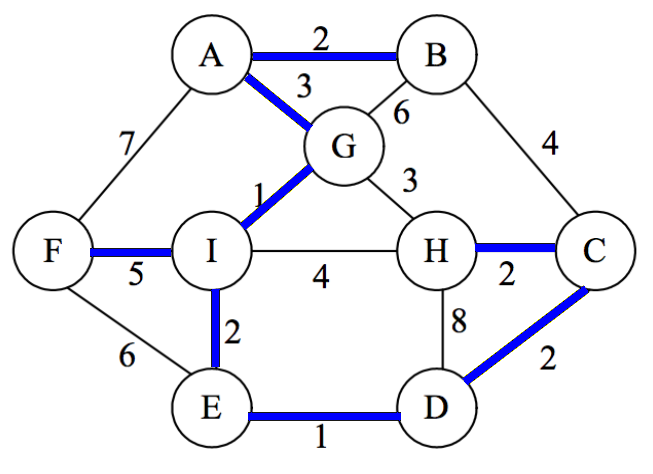
\includegraphics[width=1.5in]{final/prim-weighted-mst.png}}
\caption{\label{fig:prim-weighted-mst} MST edges shown in blue.}
\end{figure}

{\scriptsize
{\em Grading.} 
\begin{itemize}
\item Incorrectly adding up weights could subtract $1$ or $2$ points from the total.
\item Adding $9$ edge weights (or any other number instead of $8$ weights) and getting incorrect sum is $11$ points (instead of $15$). 
\item Not showing the edges in answers (or displaying them in an order that differs from Prim's algorithm), 
but still getting something close to MST is about $8$ points.
\end{itemize}
}


\end{document}

